\section{Literature Review}
	\label{sec:revBibli}
	
	\subsection{Brain-Computer Interface and EEG}
		\par Among the methods of Brain-Computer Interface (BCI), Electroencephalogram (EEG) stands out as the most cost-effective and simple system to implement. However, it does have some quirks, such as high sensitivity to electromagnetic interference and difficulty in capturing the signal due to suboptimal scalp placement of the electrodes. So one of the fundamental aspect that any EEG processing system must have is the tolerance to noise \cite{JALALYBIDGOLY2020101788}.
		
		\par The \textit{wet} electrodes are placed using conductive gel and are less prone to movement artifacts which are electromagnetic interferences caused by some motion like blinking. \textit{Dry} electrodes does not need the gel but is more sensible to artifacts.
		
		\par EEG records the electrical activities of the brain, typically placing along the scalp surface electrodes. These electrical activities result from ionic current flows induced by the synchronized synaptic activation of the brain's neurons. They manifest as rhythmic voltage fluctuations ranging from 5 to 100$\mu V$ in amplitude and between 0.5 and 40 Hz in frequency\cite{JALALYBIDGOLY2020101788}. The operational frequencies bands in the brain are following \cite{sanei2021eeg}:
		
		\begin{itemize}
			\item \textbf{Delta (1–4Hz)}: The slowest and usually the highest amplitude waveform. The Delta band is observed in babies and during deep sleep in adults.
			
			\item \textbf{Theta (4–8Hz)}: Observed in children, drowsy adults, and during memory recall. Theta wave amplitude is typically less than 100$\mu V$.
			
			\item \textbf{Alpha (8–12Hz)}: Usually the dominant frequency band, appearing during relaxed awareness or when eyes are closed. Focused attention or relaxation with open eyes reduces the amplitude of the Alpha band. These waves are normally less than 50 $\mu V$.
			
			\item \textbf{Beta (12–25Hz)}: Associated with thinking, active concentration, and focused attention. Beta wave amplitude is normally less than 30 $\mu V$.
			
			\item \textbf{Gamma (over 25Hz)}: Observed during multiple sensory processing. Gamma patterns have the lowest amplitude.
		\end{itemize}

		\par According to \cite{JALALYBIDGOLY2020101788}, for most of the tasks brain do, there are regions associated with it as seen in Table \ref{tb:brainRegions}.
	
		\begin{table}[H]
			\begin{center}
				\caption{Brain tasks and its corresponding regions. See Figure \ref{fig:1020standardandlobes} for more information.}
				\begin{tabular}{|c|c|p{0.4\textwidth}|}
					\hline
					Region & Channels & Tasks\\
					\hline
					Frontal lobe & Fp1, Fp2, Fpz, Pz, F3, F7, F4, F8 & Memory, concentration, emotions.\\
					\hline
					Parietal lobe& P3, P4, Pz & Problem Solving, attention, grammar, sense of touch. \\
					\hline
					Temporal lobe& T3, T5, T4, T6 & Memory, recognition of faces, hearing, word and social clues. \\
					\hline
					Occipital lobe & O1, O2, Oz & Reading, vision.\\
					\hline
					Cerebellum && Motor control, balance. \\
					\hline
					Sensorimotor Cortex & C3, C4, Cz& Attention, mental processing, fine motor control, sensory integration. \\
					\hline
				\end{tabular}
				\label{tb:brainRegions}
			\end{center}
		\end{table}
	
		\begin{figure}[H]
			\centering
			\includegraphics[width=0.44\linewidth]{images/10–20StandardAndLobes}
			\caption[10-20 standard and brain lobes]{Electrodes placement according to 10-20 standard \cite{sistema10-20} and brain's lobes. Odd numbers are assigned to the electrodes on the left hemisphere, and even numbers are assigned to the electrodes on the right. Source \cite{JALALYBIDGOLY2020101788}}
			\label{fig:1020standardandlobes}
		\end{figure}
	
	\subsection{Spiking Neural Networks}
	
		\par Neural Networks (NNs), as defined here as \textit{a multilayered, fully connected, with or without recurrent or convolutional layers network}, require that all neurons are activated in both the forward and backward passes. This implies that every unit in the network must process some data, leading to power consumption \cite{10242251}. 

		\par The sensory system of biological neurological systems converts external data, such as light, odors, touch, flavors, and others, into \textbf{spikes}. A spike is a voltage that convey information \cite{kasabov2019time}. These ones are then transmitted along the neuronal chain to be processed, generating a response to the environment.
		
		\par The biological neuron only spikes when a certain level of excitatory signals get accumulated above some threshold in its soma staying inactive when there is no signal, therefore, this type of cell is very efficient in terms of energy consumption and processing.
		
		\par In order to get the aforementioned advantages the Spiking Neural Networks (SNNs) instead of employing continuous activation values, like NNs, SNNs utilize \textbf{spikes} at the input, hidden and outputs layers. SNNs can have continuous inputs as well and keep its properties.
		
		
		\par An SNN \textbf{is not} a one-to-one simulation of neurons. Instead, it approximates certain computational capabilities of specific biological properties. Some studies like \cite{jones2020single} created models way closer to natural neurons exploring the nonlinearity of dendrites and another neuron features yielding remarkable results in the classification.
		
		\begin{multicols}{2}
			\par As can be seen in Figure \ref{fig:neuronspike} SNNs neurons, given the correct parameters, are very noise tolerant because it acts as a \textbf{lowpass filter}. Generating spikes even when a considerably level of interference is present. This units are very time-oriented too, being great when it comes to process streams of data \cite{10242251}.
		\columnbreak
			\begin{figure}[H]
				\centering
				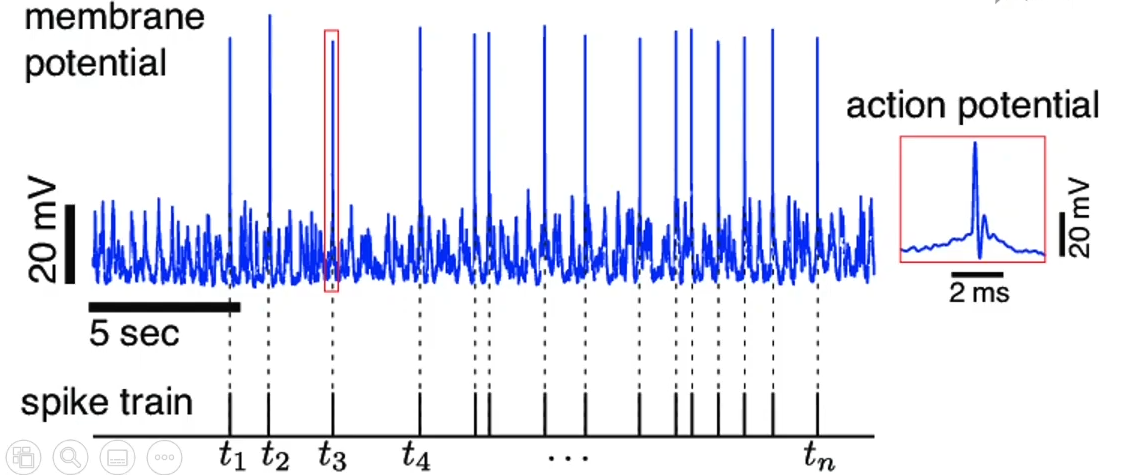
\includegraphics[width=.88\linewidth]{images/neuronSpikes}
				\caption{Spikes from a noisy signal. Source \cite{dan_goodman_2022_7044500}}
				\label{fig:neuronspike}
			\end{figure} 
		\end{multicols}

	\subsection{Spiking Neuron}
		\par Although this work focus in just \textit{Leaky Integrate and Fire Neurons} (LIF) because is simpler, more efficient and currently generalize better for most of the problems \cite{dan_goodman_2022_7044500}, there is one interesting enough, because it paves the way to another ones, that worth to mention:
	
		\subsubsection{Hodgkin-Huxley neuron}
			\par The Hodgkin-Huxley neuron \cite{gerstner2014neuronal} was modeled conducting experiments on a giant axon of a squid and identified three distinct types of ion currents: $Na^+$ (sodium), $K^+$ (Potassium), and a leak current primarily composed of $Cl^-$ (chloride) ions.
			
			
			\begin{multicols}{2}
				\par Like can be seen in Figure \ref{fig:hodgkin-huxleymodel} this neuron is modeled as conjunction of a resistor $R$, potentiometers $R_{Na}, R_{K}$ and a capacitor $C$ along with  batteries (ion concentrators) $E_L, E_{Na}, E_K$  in which an current $I$ is injected. The potentiometers indicate the channels of $Na^+$ and $K^+$ which can ben opened or closed, the batteries represents Nernst potential \cite{2023Gibbs} for each channel.
			\columnbreak
				\begin{figure}[H]
					\centering
					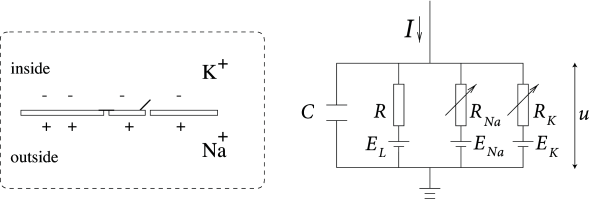
\includegraphics[width=0.5\linewidth]{images/Hodgkin-HuxleyModel}
					\caption{Schematic diagram for the Hodgkin-Huxley model. Source: \cite{gerstner2014neuronal}}
					\label{fig:hodgkin-huxleymodel}
				\end{figure}
			\end{multicols}
			
			\par Given that:
			\begin{itemize}
				\item $C_m$ is the membrane capacitance that represents the ability of the neuronal membrane to store charge.
				\item $g_{Na}$ is the sodium conductance that describes its fast opening permeability.
				\item $g_K$ is the potassium conductance that describes its slow opening permeability.
				\item $g_{leak}$ is the background conductance that describes ion movements not related to $Na^+$ or $K^+$ channels.
				\item $V$ is the membrane potential.
				\item $I$ is the injected current.
				\item $m, h$, and $n$ are dimensionless gating variables representing the probability that the sodium and potassium channels are open.
				\item $\alpha$ and $\beta$ are voltage-dependent rate constants.
			\end{itemize}
		
			\par Than the neuron's behavior is ruled by the Equations \ref{eq:Hodgkin-HuxleyNeuronEq1}, \ref{eq:Hodgkin-HuxleyNeuronEq2}, \ref{eq:Hodgkin-HuxleyNeuronEq3}, \ref{eq:Hodgkin-HuxleyNeuronEq4} and Listings \ref{lst:hodgkin-huxleymodelLst1}, \ref{lst:hodgkin-huxleymodelLst02-04}, \ref{lst:hodgkin-huxleymodelHelper}.\newline
			
			\par The equation \ref{eq:Hodgkin-HuxleyNeuronEq1} models how rate of change $\frac{dV}{dt}$ of membrane potential ($V$) is determined by the injected current ($I$) and the currents through $Na^+$, $K^+$, and $g_{leaky}$ channels.
			\begin{equation}
				\label{eq:Hodgkin-HuxleyNeuronEq1}
				\frac{dV}{dt} = \dfrac{I - g_{\text{Na}}m^3h(V - E_{\text{Na}}) - g_{\text{K}}n^4(V - E_{\text{K}}) - g_{\text{leak}}(V - E_{\text{leak}})}{C_m}
			\end{equation}
			\begin{lstlisting}[language=Python, caption={Python implementation of the Hodgkin-Huxley neuron's first equation}, label={lst:hodgkin-huxleymodelLst1}]
# Equation 1
dVdt = (I_total - I_Na - I_K - I_leak) / Cm
\end{lstlisting}
	
	
	
	
	
			\begin{multicols}{2}
			
				\par Equations \ref{eq:Hodgkin-HuxleyNeuronEq2}, \ref{eq:Hodgkin-HuxleyNeuronEq3}, \ref{eq:Hodgkin-HuxleyNeuronEq4} are the rate of change of the gating variables $m, h$, and $n$, which represent the probability that the $Na^+$ and $K^+$ channels are open.
				\begin{lstlisting}[language=Python, caption={Python implementation of the Hodgkin-Huxley neuron's second, third and fourth equation}, label={lst:hodgkin-huxleymodelLst02-04}]
# Equations 2-4
dmdt = alpha_m(V) * (1 - m) - beta_m(V) * m
dhdt = alpha_h(V) * (1 - h) - beta_h(V) * h
dndt = alpha_n(V) * (1 - n) - beta_n(V) * n
\end{lstlisting}
	
			\columnbreak
	
				\begin{equation}
					\label{eq:Hodgkin-HuxleyNeuronEq2}
					\frac{dm}{dt} = \alpha_m (1 - m) - \beta_m m
				\end{equation}
			
				\begin{equation}
					\label{eq:Hodgkin-HuxleyNeuronEq3}
					\frac{dh}{dt} = \alpha_h (1 - h) - \beta_h h
				\end{equation}
			
				\begin{equation}
					\label{eq:Hodgkin-HuxleyNeuronEq4}
					\frac{dn}{dt} = \alpha_n (1 - n) - \beta_n n
				\end{equation}
			
			\end{multicols}
			
			\begin{multicols}{2}
				\par The helper functions representing the $\alpha$ and $\beta$ are used to calculate the rate constants for the gating variables in the differential equations.	
				\begin{lstlisting}[language=Python, caption={Helper functions representing the $\alpha$ and $\beta$}, label={lst:hodgkin-huxleymodelHelper}]
# Helper functions for rate constants
def alpha_m(V):
	return 0.1 * (V + 40.0) / (1.0 - math.exp(-(V + 40.0) / 10.0))
def beta_m(V):
	return 4.0 * math.exp(-(V + 65.0) / 18.0)
def alpha_h(V):
	return 0.07 * math.exp(-(V + 65.0) / 20.0)
def beta_h(V):
	return 1.0 / (1.0 + math.exp(-(V + 35.0) / 10.0))
def alpha_n(V):
	return 0.01 * (V + 55.0) / (1.0 - math.exp(-(V + 55.0) / 10.0))
def beta_n(V):
	return 0.125 * math.exp(-(V + 65.0) / 80.0)
\end{lstlisting}
			\columnbreak
				\begin{equation}
					\alpha_m(V) = 0.1 \frac{V + 40.0}{1.0 - \exp\left(-\frac{V + 40.0}{10.0}\right)}
				\end{equation}
			
				\begin{equation}
					\beta_m(V) = 4.0 \exp\left(-\frac{V + 65.0}{18.0}\right)
				\end{equation}
			
				\begin{equation}
					\alpha_h(V) = 0.07 \exp\left(-\frac{V + 65.0}{20.0}\right)
				\end{equation}
			
				\begin{equation}
					\beta_h(V) = \frac{1.0}{1.0 + \exp\left(-\frac{V + 35.0}{10.0}\right)}
				\end{equation}
			
				\begin{equation}
					\alpha_n(V) = 0.01 \frac{V + 55.0}{1.0 - \exp\left(-\frac{V + 55.0}{10.0}\right)}
				\end{equation}
		
				\begin{equation}
					\beta_n(V) = 0.125 \exp\left(-\frac{V + 65.0}{80.0}\right)
				\end{equation}
			\end{multicols}
			
			\begin{figure}[H]
				\centering
				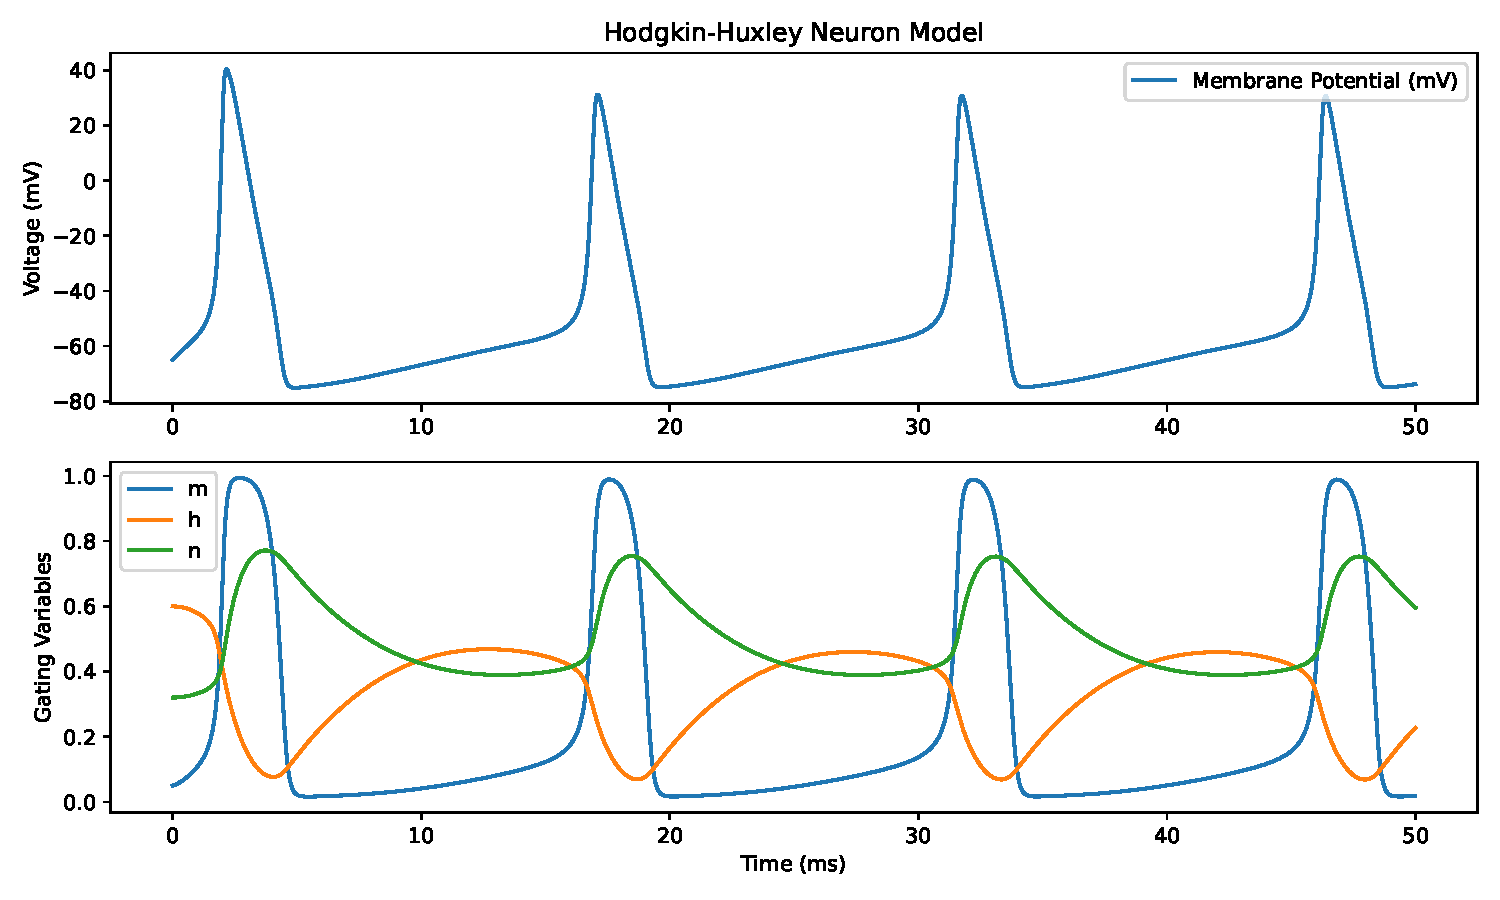
\includegraphics[width=0.7\linewidth]{images/hodkinHuxleyNeuronBehavior}
				\caption[Hodgkin-Huxley neuron behavior]{Hodgkin-Huxley neuron behavior under constant input current. Source: The author}
				\label{fig:hodkinhuxleyneuronbehavior}
			\end{figure}
			
			\par The full code that plots the Figure \ref{fig:hodkinhuxleyneuronbehavior} which shows the neuron behavior is shown in Listing \ref{lst:Hodkin-Huxley}.
			\begin{lstlisting}[language=Python, caption={Full implementation of a Hodkin-Huxley neuron}]
import math
import matplotlib.pyplot as plt

# Hodgkin-Huxley model parameters
Cm = 1.0   # Membrane capacitance (uF/cm^2)
g_Na = 120.0  # Sodium conductance (mS/cm^2)
g_K = 36.0    # Potassium conductance (mS/cm^2)
g_leak = 0.3  # Leak conductance (mS/cm^2)
E_Na = 50.0   # Sodium reversal potential (mV)
E_K = -77.0   # Potassium reversal potential (mV)
E_leak = -54.387  # Leak reversal potential (mV)

# Time parameters
dt = 0.01  # Time step (ms)
t_max = 50.0  # Maximum simulation time (ms)

# Initial conditions
V, m, h, n = -65.0, 0.05, 0.6, 0.32  # V, m, h, n

# Lists to store results for plotting
time_points = []
membrane_potential = []
gating_variables_m = []
gating_variables_h = []
gating_variables_n = []

# Helper functions for rate constants
def alpha_m(V):
	return 0.1 * (V + 40.0) / (1.0 - math.exp(-(V + 40.0) / 10.0))

def beta_m(V):
	return 4.0 * math.exp(-(V + 65.0) / 18.0)

def alpha_h(V):
	return 0.07 * math.exp(-(V + 65.0) / 20.0)

def beta_h(V):
	return 1.0 / (1.0 + math.exp(-(V + 35.0) / 10.0))

def alpha_n(V):
	return 0.01 * (V + 55.0) / (1.0 - math.exp(-(V + 55.0) / 10.0))

def beta_n(V):
	return 0.125 * math.exp(-(V + 65.0) / 80.0)

# Simulation loop
for t in range(int(t_max / dt)):
	# Membrane currents
	I_Na = g_Na * m**3 * h * (V - E_Na)
	I_K = g_K * n**4 * (V - E_K)
	I_leak = g_leak * (V - E_leak)
	
	# Total membrane current
	I_total = 10.0  # Injected current (adjust as needed)
	
	# Update variables using Euler method
	dVdt = (I_total - I_Na - I_K - I_leak) / Cm
	dmdt = alpha_m(V) * (1 - m) - beta_m(V) * m
	dhdt = alpha_h(V) * (1 - h) - beta_h(V) * h
	dndt = alpha_n(V) * (1 - n) - beta_n(V) * n
	
	V += dt * dVdt
	m += dt * dmdt
	h += dt * dhdt
	n += dt * dndt
	
	# Store results for plotting
	time_points.append(t * dt)
	membrane_potential.append(V)
	gating_variables_m.append(m)
	gating_variables_h.append(h)
	gating_variables_n.append(n)

# Plot results
plt.figure(figsize=(10, 6))
plt.subplot(2, 1, 1)
plt.plot(time_points, membrane_potential, label='Membrane Potential (mV)')
plt.title('Hodgkin-Huxley Neuron Model')
plt.ylabel('Voltage (mV)')
plt.legend()

plt.subplot(2, 1, 2)
plt.plot(time_points, gating_variables_m, label='m')
plt.plot(time_points, gating_variables_h, label='h')
plt.plot(time_points, gating_variables_n, label='n')
plt.xlabel('Time (ms)')
plt.ylabel('Gating Variables')
plt.legend()

plt.tight_layout()
plt.show()

\end{lstlisting}

			

		\subsubsection{Leaky Integrate and Fire Neuron}
			\par The Leaky Integrate and Fire Neuron (LIF) is one of the simplest neuron models in SNNs, still, it can applied successfully to most of the problems in with SNNs can be used.
			\begin{multicols}{2}
				\par LIF, like a NN neuron takes the sum of weighted inputs but, rather than pass it directly to its activation function, some \textit{leakage} is applied, which decreases in some degree the sum. 
				\par LIF behave much like Resistor-Capacitor circuits as can be seen in Figure \ref{fig:rcmodel}. Here $R$ is resistance to the leakage, $I_{in}$ the input current, $C$ the capacitance, $U_{mem}$ means the accumulated action potential and $v$ is a switch that lets the capacitor discharge (i.e. emit a spike) when some potential threshold is reached.
			\columnbreak
				\begin{figure}[H]
					\centering
					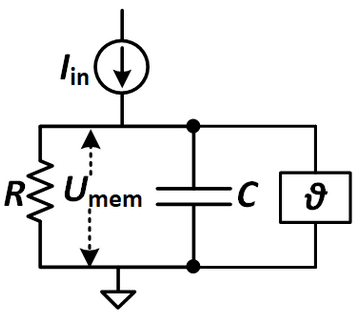
\includegraphics[width=0.5\linewidth]{images/rcmodel}
					\caption[The RC model]{RC model: Source: \cite{10242251}}
					\label{fig:rcmodel}
				\end{figure}
			\end{multicols}
			
			\par Unlike the Hodgkin-Huxley neuron, spikes are represented as \textbf{sparsely} distributed \textbf{ones} in a train of \textbf{zeros}, as illustrated in Figure \ref{fig:spikessparsitystaticsupress} and \ref{fig:sparsity}. This approach simplify the models and reduces the computational power and needed storage to run an SNN.\newline
			
			\begin{multicols}{2}
				\begin{figure}[H]
					\centering
					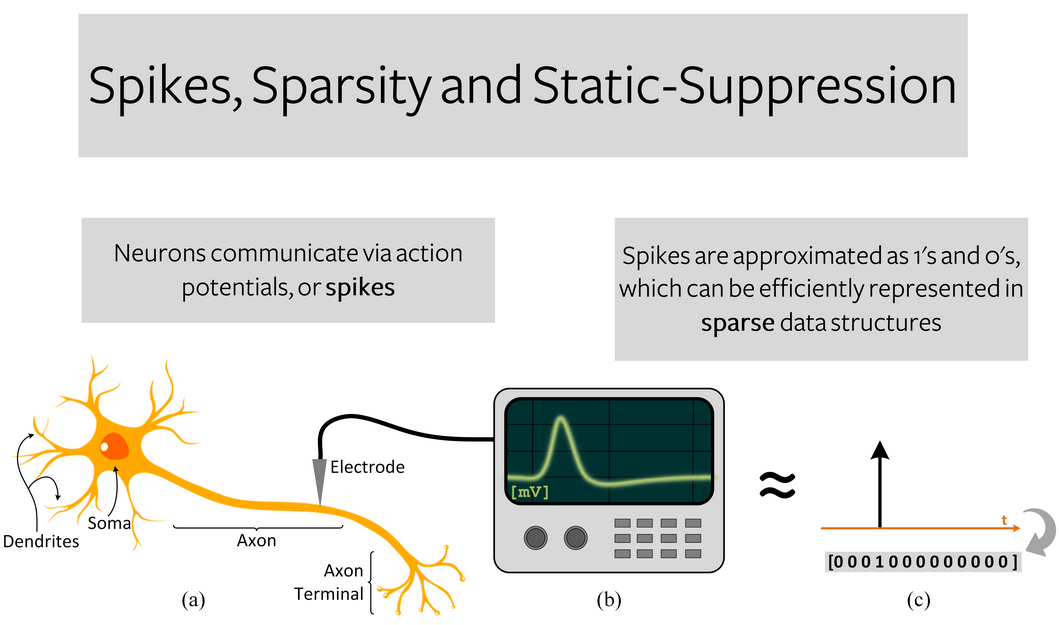
\includegraphics[width=\linewidth]{images/spikesSparsityStaticSupress}
					\caption{Sparsity on Spike Neuron Networks. Source: \cite{10242251}}
					\label{fig:spikessparsitystaticsupress}
				\end{figure}
			\columnbreak
				\begin{figure}[H]
					\centering
					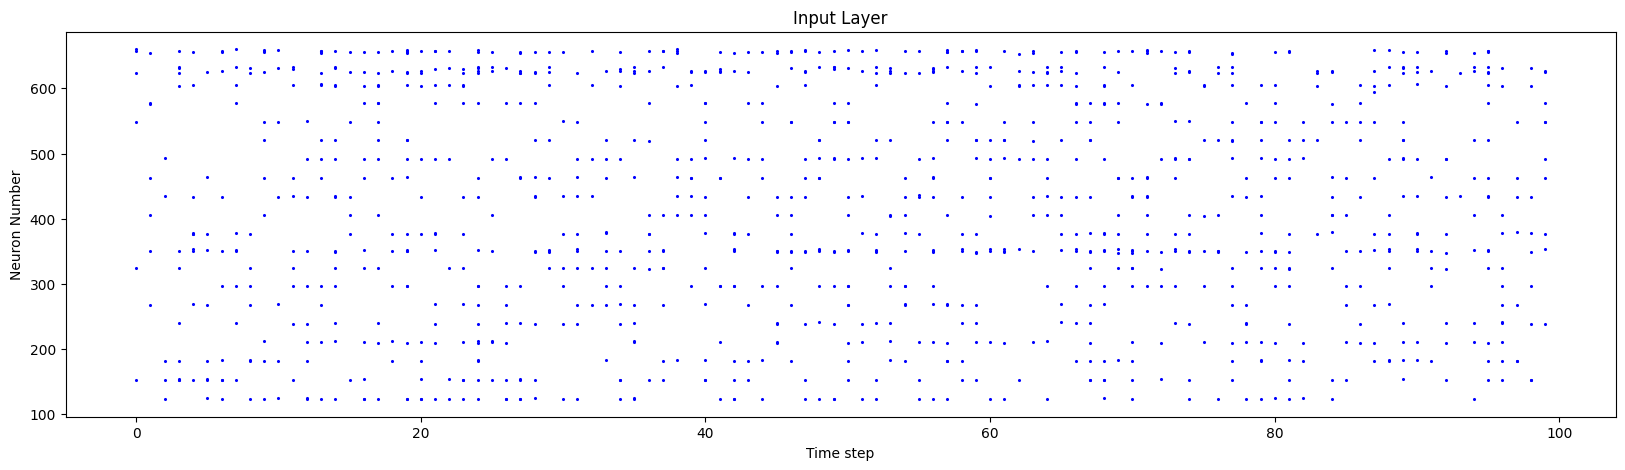
\includegraphics[width=.5\linewidth]{images/sparsity}
					\caption[Sparse activity of a SNN]{Sparse activity of a SNN: The horizontal axis represents the time step of some data being processed the vertical are the SNN neuron number. Note that, most of the time, very few neurons gets activated. Source: The author.}
					\label{fig:sparsity}
				\end{figure}
			\end{multicols}
				
			\par As result of the mentioned above, in SNN information is coded in format of \textit{timing} and/or \textit{rate} of spikes giving consequently great capabilities of processing streams of data but limiting the processing of static data.\newline
			
			\par LIF model is governed by the Equations bellow \cite{10242251}.\newline
			
			
			\par Considering that $Q$ is a measurement of electrical charge and $V_{mem}(t)$ is the potential difference at the membrane in a certain time $t$ than the neuron capacitance $C$ is given by the Equation \ref{eq:capacitance}.
			
			\begin{equation}
				\label{eq:capacitance}
				C = \frac{Q}{V_{mem}(t)}
			\end{equation}
			
			\par Than the neuron charge can be expressed as Equation \ref{eq:charge}.
			
			\begin{equation}
				\label{eq:charge}
				Q = C.V_{mem}(t)
			\end{equation}
		
			\par To know how these charge changes according to the time (aka current) we can derivate $Q$ as in Equation \ref{eq:rateOfChargeChange}. This expression express the current in the capacitive part of the neuron $I_C$
			
			\begin{equation}
				\label{eq:rateOfChargeChange}
				I_C = \dfrac{dQ}{dt} = C. \dfrac{dV_{mem}(t)}{dt}
			\end{equation}
		
		
			\par To calculate the total current passing by the resistive part of the circuit we may use the Ohm's law:
			
			\begin{equation}
				\label{eq:ohmlaw}
				V_{mem}(t) = R.I_R \implies I_R = \frac{V_{mem}(t)}{R}
			\end{equation}
			
			\par Than considering that the total current do not change, as seen in Figure \ref{fig:rcmodel2}, we have the total input current $I_{in}$ of the neuron as in Equation \ref{eq:totalNeuronCurrent}.
			
			\begin{multicols}{2}
			
				\begin{figure}[H]
					\centering
					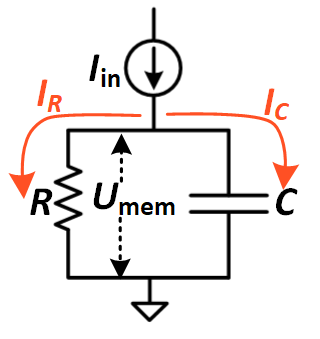
\includegraphics[width=0.4\linewidth]{images/rcmodel2}
					\caption[RC model for currents]{RC model for currents: $I_{in} = I_R + I_C$}
					\label{fig:rcmodel2}
				\end{figure}
			
			\columnbreak
		
				\begin{equation}
					\label{eq:totalNeuronCurrent}
					I_{in}(t) = I_R + I_C \implies I_{in}(t) = \frac{V_{mem}(t)}{R} + C.\dfrac{dV_{mem}(t)}{dt}
				\end{equation}
			\end{multicols}
		
			\par Therefore, to describe the passive membrane we got a linear Equation \ref{eq:memLinear}.
			
			\begin{equation}
				\label{eq:memLinear}
				\begin{aligned}
					I_{in}(t) &= \frac{V_{mem}(t)}{R} + C.\dfrac{dV_{mem}(t)}{dt} \implies \\ 
					I_{in}(t) - \frac{V_{mem}(t)}{R} &=  C.\dfrac{dV_{mem}(t)}{dt} \implies \\
					\Aboxed{R.I_{in}(t) - V_{mem}(t) &=  R.C.\dfrac{dV_{mem}(t)}{dt}}
				\end{aligned}
			\end{equation}
		
			\par Than, if we consider $\tau = R.C$ as the \textbf{membrane time constant} we get voltages on both sides of Equation \ref{eq:finalMem} which \textbf{describes the RC circuit}.
			
			\begin{equation}
				\label{eq:finalMem}
				\begin{aligned}
				R.I_{in}(t) - V_{mem}(t) &=  R.C.\dfrac{dV_{mem}(t)}{dt} \implies \\
				R.I_{in}(t) - V_{mem}(t) &=  \tau.\dfrac{dV_{mem}(t)}{dt} \implies \\
				\Aboxed{\tau.\dfrac{dV_{mem}(t)}{dt} &= R.I_{in}(t) - V_{mem}(t)}
				\end{aligned}
			\end{equation}
		
			\par From that, and setting $I_{in} = 0$ (i.e. no input) and considering $\tau = R.C$ is a constant and an starting voltage $V_{mem}(0)$ the neuron's voltage behavior can be modeled as an exponential curve as can be seen in Equation \ref{eq:expmembrane}.
		
		 	\begin{equation}
		 		\label{eq:expmembrane}
		 		\begin{aligned}
		 		\tau.\dfrac{dV_{mem}(t)}{dt} &= R.I_{in}(t) - V_{mem}(t) \implies \\
		 		\tau.\dfrac{dV_{mem}(t)}{dt} &= -V_{mem}(t) = \\
		 		e^{\ln(V_{mem}(t))} &= e^{-\frac{t}{\tau}} = \\
		 		\Aboxed{V_{mem}(t) &= V_{mem}(0).e^{-\frac{t}{\tau}}}
		 		\end{aligned}
		 	\end{equation}
	 	
	 		\par Then one can say that: In the absence of an input $I_{in}$, the membrane potential decays exponentially as illustrated in Figure \ref{fig:membranepotentialdecay} and implemented in Listing \ref{lst:membranepotentialdecay}.
	 		
	 		\begin{multicols}{2}
	 			\begin{lstlisting}[language=Python, caption={Python implementation of the action potential decaying of a LIF: $I_{in} = 0$}, label={lst:membranepotentialdecay}]
def lif(V_mem, dt=1, I_in=0, R=5, C=1):
	tau = R*C
	V_mem = V_mem + (dt/tau)*(-V_mem + I_in*R)
	return V_mem
\end{lstlisting}
	 		\columnbreak
		 		\begin{figure}[H]
		 			\centering
		 			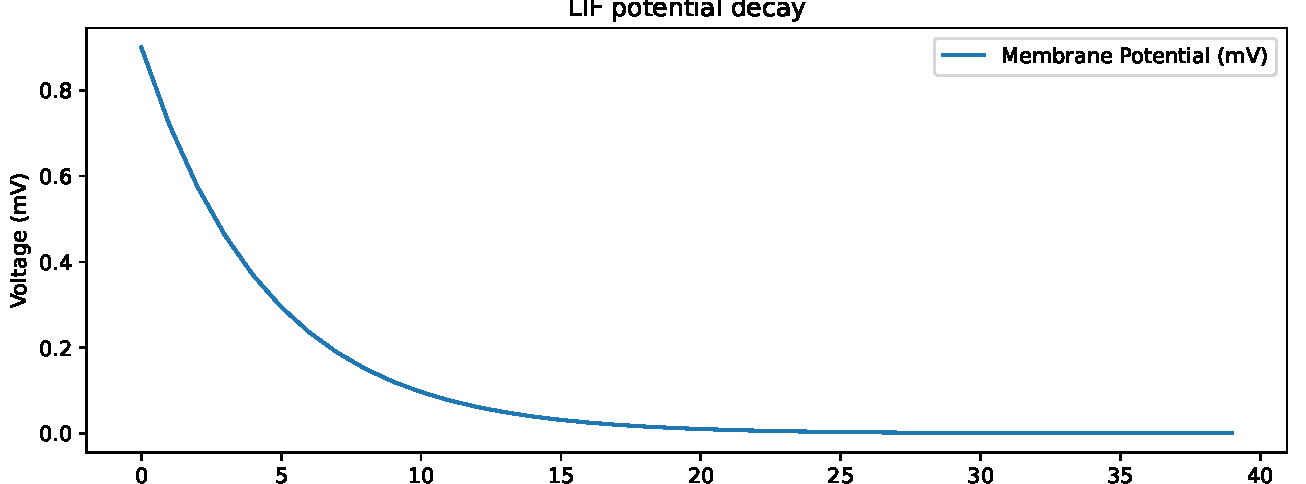
\includegraphics[width=\linewidth]{images/membranePotentialDecay}
		 			\caption{Membrane potential decaying. Source: The author}
		 			\label{fig:membranepotentialdecay}
		 		\end{figure}
	 		\end{multicols}
 			
 			\par With the results from Equation \ref{eq:finalMem} it is possible to calculate the action potential increasing as seen in Equation \ref{eq:actionpotincrease}.
 			
 			\begin{equation}
 				\label{eq:actionpotincrease}
 				\begin{aligned}
 					&\tau.\dfrac{dV_{mem}(t)}{dt} = R.I_{in}(t) - V_{mem}(t) = \\
 					&\tau.\dfrac{dV_{mem}(t)}{dt} + V_{mem}(t) = R.I_{in}(t) = \\
 					&\dfrac{dV_{mem}(t)}{dt} + \frac{V_{mem}(t)}{\tau} = \frac{R.I_{in}(t)}{\tau} \implies \\
 					&\text{Integrating factor: } e^{\int \frac{1}{\tau} dt} = e^{\frac{1}{\tau}.t} \implies \\
					&(e^{\frac{1}{\tau}.t}.V_{mem}(t))' = \frac{R.I_{in}(t)}{\tau}.e^{\frac{1}{\tau}.t} = \\
					&\int (e^{\frac{1}{\tau}.t}.V_{mem}(t))' = \int \frac{R.I_{in}(t)}{\tau}.e^{\frac{1}{\tau}.t} dt = \\
					&e^{\frac{1}{\tau}.t}.V_{mem}(t) = \int \frac{R.I_{in}(t)}{\tau}.e^{\frac{1}{\tau}.t} dt \therefore \\
					& \text{Considering: } V_{mem}(t=0) = 0 \implies \\
					\Aboxed{&V_{mem}(t) = I_{in}(t).R(1-e^{\frac{1}{\tau}})}
 				\end{aligned}
 			\end{equation}
 		
 			\par Note that when action potentials increases there is still an exponential behavior as seen in Figure \ref{fig:membranepotentialincrease} and implemented in Listing \ref{lst:membranepotentialincrease}.
 			
 			\begin{lstlisting}[language=Python, caption={Python implementation of the action potential decreasing of a LIF: $I_{in}=1$}, label={lst:membranepotentialincrease}]
	
def lif(V_mem, dt=1, I_in=1, R=5, C=1):
	tau = R*C
	V_mem = V_mem + (dt/tau)*(-V_mem + I_in*R)
	return V_mem
\end{lstlisting}

 			\begin{figure}[H]
 				\centering
 				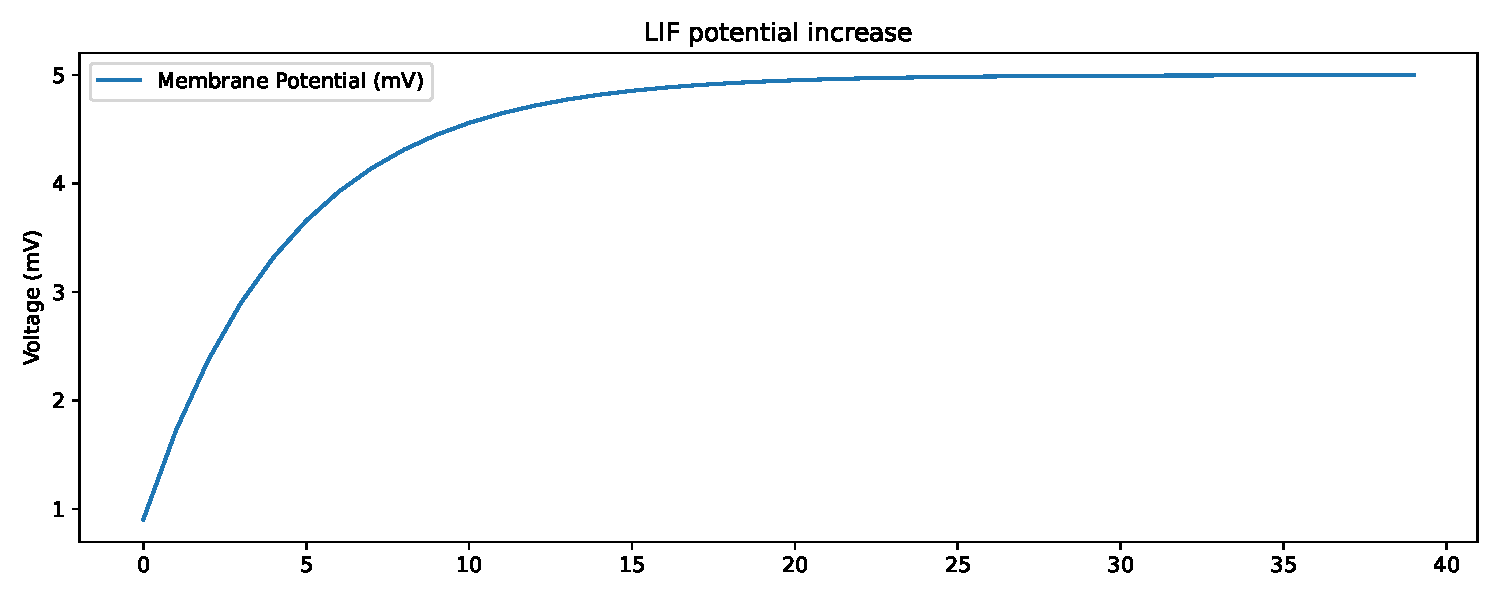
\includegraphics[width=0.7\linewidth]{images/membranePotentialIncrease}
 				\caption{Membrane potential increasing. Source: The author}
 				\label{fig:membranepotentialincrease}
 			\end{figure}
 		
 			\par Then taking into account some \textbf{threshold} which indicates a reset into the neuron potential and two type of resets (to zero and threshold subtraction) finally is possible to make a full simulation depicted in Figure \ref{fig:membranepotentialfull} and implemented in Listing \ref{lst:membranepotentialfull}:
 			
 			\begin{lstlisting}[language=Python, caption={Python implementation of the action potential full simulation of a LIF: $I_{in}=1$, $V_{thresh} = 2$ is threshold}, label={lst:membranepotentialfull}]
def lif(V_mem, dt=1, I_in=1, R=5, C=1, V_thresh = 2, reset_zero = True):
	tau = R*C
	V_mem = V_mem + (dt/tau)*(-V_mem + I_in*R)
	if V_mem > V_thresh:
		if reset_zero:
			V_mem = 0
		else:
			V_mem = V_mem - V_thresh
	return V_mem
\end{lstlisting}

 			
 			\begin{figure}[H]
 				\centering
 				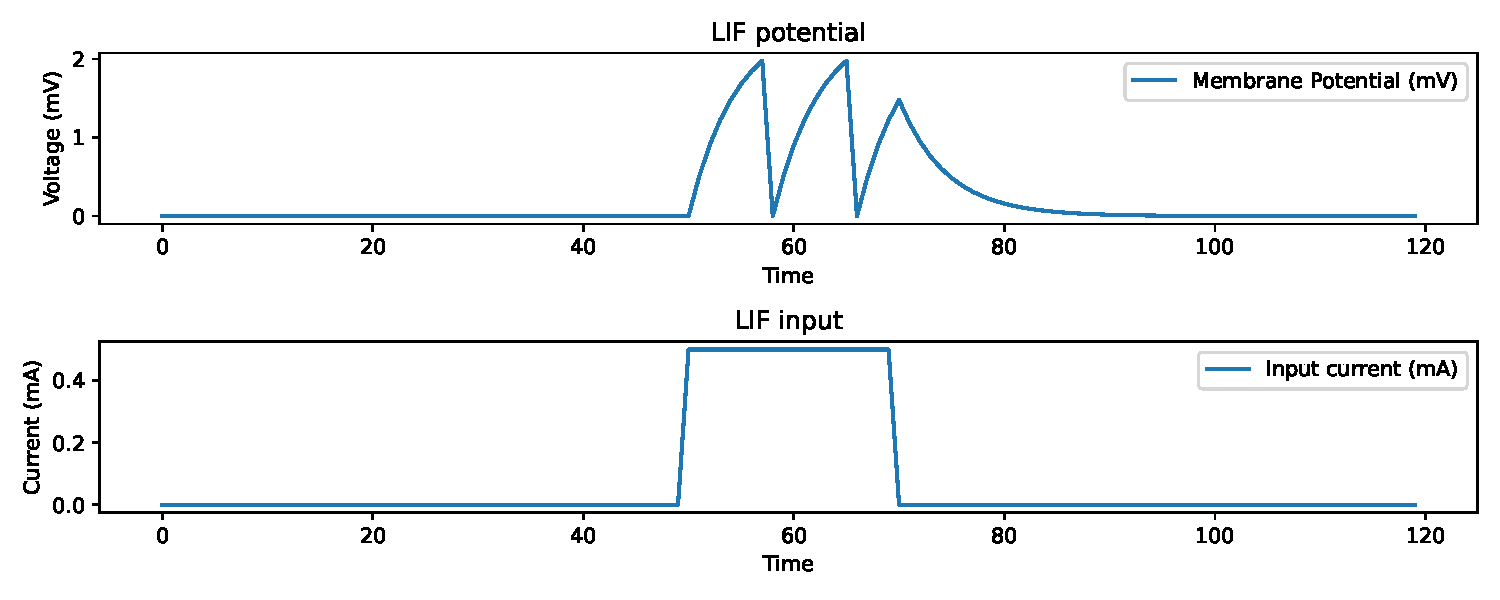
\includegraphics[width=0.8\linewidth]{images/membranePotentialFull}
 				\caption{Plot of the full simulated LIF: A 0.5 mA was provided from time 51 to 70.}
 				\label{fig:membranepotentialfull}
 			\end{figure}
 			
 			
			
			
			
			
			
			
			
			
			
			
			
			
			
			
			




